

\section{Vectorization}

\subsubsection*{Multiple instruction - single data:}

Vectorization means organizing the routines in such a way that many operations can be done simultaneously. Vectorization only works in the innermost loops. As an example

\small
\begin{lstlisting}[frame=single]

i_max = 10000;
for(i=1; i<=i_max; i++){

	A(i) = B(i) * (C(i) + D(i));

}
\end{lstlisting}
\normalsize
In the loop, one has to do several operations: fetch the values of the vectors A,B,C,D, multiply them, adding etc. ... The aim is to parallelize all these operations in a pipe. This is usually already implemented in the compilers, so that the user does not have to care about it. In more complicated routines this may have to be implemented directly. The bad features for vectorization of a routine include

\begin{itemize}
\item Short loops.
\item Conditional branchings like if-statements.
\item Indirect addressing.
\end{itemize}

If the loop is smaller than the ``assembly line'' then there's no need to bother programming in a vectorized way (i.e. if $i_max$ in the upper example would be 4 or 5). Another problem is that the instructions must be repetitive without interruptions or exceptions like if-statements. There are ways to handle some cases in which a distinction is needed, but this is often a problem. An example would be replacing 
\small
\begin{lstlisting}[frame=single]
if(P(i)>z){
	s = -s;
}
\end{lstlisting}
\normalsize
by
 \small
\begin{lstlisting}[frame=single]
s = s*sign(z-P(i));
\end{lstlisting}
\normalsize


In order for vectorization to be maximally exploited, one has to make sure that the inner loop is the largest. One can, for example, transform a n-dimensional system in a one dimensional system using helical boundary conditions and appropriate indexing. Other important elements of an efficient vectorized routine are

\begin{itemize}
\item Make update in inner loop, i.e. no loops inside this loop.
\item Use a vectorized random number generator.
\item Split up loops that cannot be vectorized.
\end{itemize}



\subsubsection*{SIMD vs MIMD:}

There are many types of parallelization, but one can roughly divide them into two groups according to the flexibility of the process and accessibility of your memory access: \emph{Single Instruction - Multiple Data} (SIMD) and \emph{Multiple Instruction - Multiple Data}. In the first case one applies the same set of instructions to all the data. In the second one, different instructions are applied to different data, with the drawback that the routines loose simplicity. There are \emph{shared memory} computers which have the advantage that they are really flexible in the organization of the data structure and \emph{distributed memory} computers which are much easier to build and program. Finally, there is the possibility of combining a great number of processors, each of them with very basic features or a smaller number of more powerful processors (\emph{coarse graining} vs \emph{fine graining}). For each combination there exist different solutions with different programming philosophies. 

\vspace{0.3cm}

$
\centering
\begin{array}{ccc}
\text{SIMD}  & \leftrightarrow  & \text{MIMD}\\
 \hline
 \text{shared memory}  & \leftrightarrow   & \text{distributed memory}\\
 \text{coarse grained}  & \leftrightarrow   & \text{fine grained}\\ 
\end{array}
$

\vspace{0.3cm}





\subsubsection*{MC parallelization:}

Monte Carlo on regular lattices is well suited for parallelization because of a number of reasons:

\begin{itemize}
\item Local processes that do not involve the whole system (nearest neighbors).
\item Domain composition is possible (sub-lattices).
\item Use standard domain decomposition and distribute using in MPI.
\item Use logical mask to extract one sub-lattice.
\item Use periodic shift (CSHIFT) to get neighbors for periodic boundary conditions.
\end{itemize}

There are many options for dividing a system  into domains. Depending on the situations it can be more convenient to increase the domains or reducing the interfaces between the domains in case that the processes need to work independently (e.g., in the case of distributed memory). It is also possible to dynamically change the size of the domains and the position of the interfaces. For an example of parallelization, see Section \ref{code:parallel_pi}.





\noindent
\begin{minipage}{\textwidth}
\begin{minipage}{.98\textwidth}
  \centering
  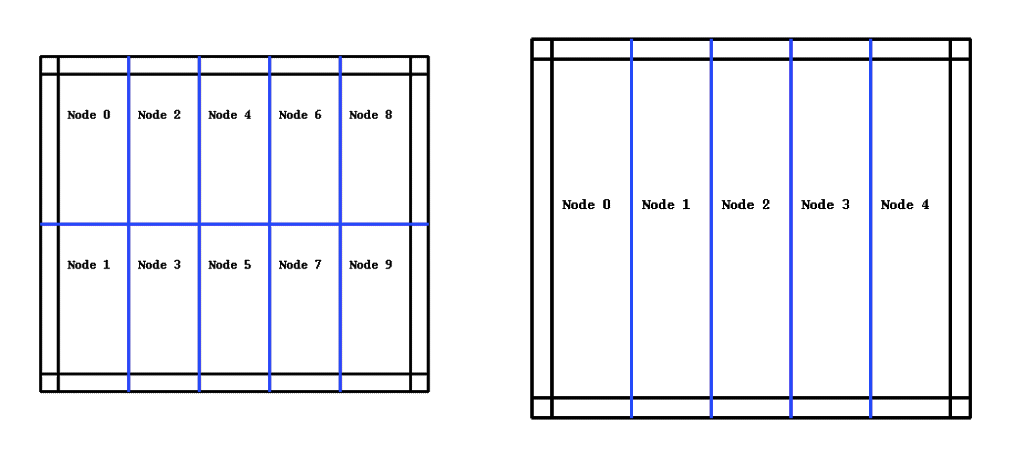
\includegraphics[height=200pt]{pics/node1}
  \captionof{figure}{Domain decomposition of a square lattice.}
  \label{fig:node1}
\end{minipage}%
\hfill
\begin{minipage}{.98\textwidth}
  \centering
  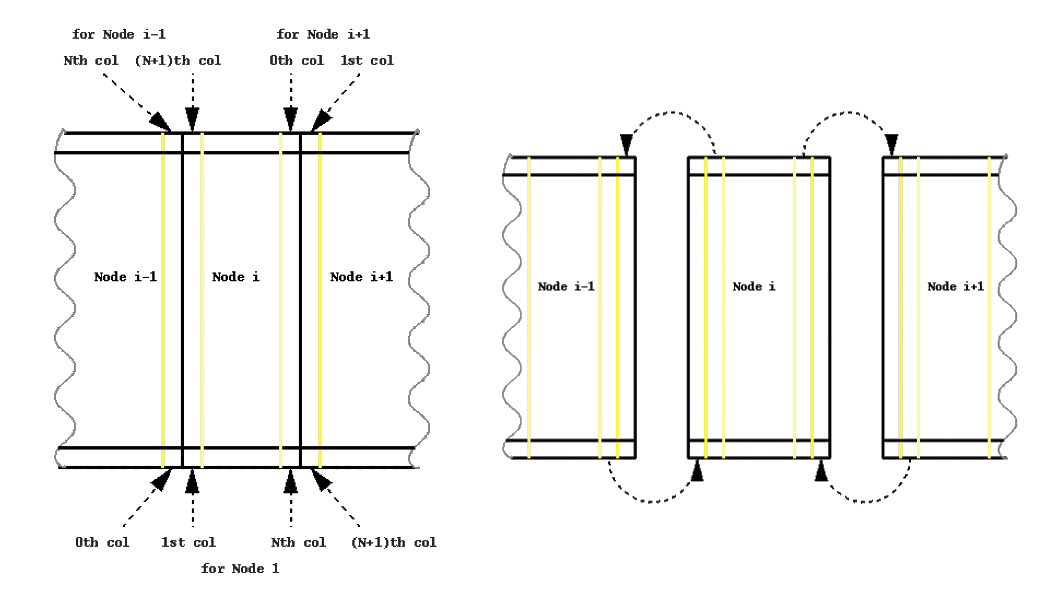
\includegraphics[height=200pt]{pics/node2}
  \captionof{figure}{Different interface setups for domain decomposition of a square lattice}
  \label{fig:node2}
\end{minipage}
\end{minipage}
\vspace{0.1cm}






\subsubsection*{Message Passing Instruction:}

To parallelize a routine one has to use specific programming languages created specifically for parallelizing or embed special libraries in which the parallelization has been implemented in such a way that it can be summoned in standard programming languages such as C++. An interesting example is CUDA (Compute Unified Device Architecture), a parallel computing platform and programming model created by NVIDIA and implemented by the graphics processing units (graphic cards) that they produce. Graphic cards are capable of very fast computation of easy operations, and that can be used in some cases to do scientific computing. \emph{Message Passing Instruction} (MPI) is a standardized and portable message-passing system. This means that instructions can be passed by the user within programs written in languages such as Java or C++. See Section \ref{code:mpi} for basic examples of MPI coding.



\subsubsection*{Amdahl's law:}

The bottleneck of parallelization is the communication between processors. Processors are not isolated units that completely work on their own, and the more one slices the system into domains, the more communication between processors is needed. This is generally not efficient and usually slows down the parallelization.


\vspace{0.1cm}
\noindent
\noindent\begin{minipage}{\textwidth}
\begin{minipage}{.98\textwidth}
  \centering
  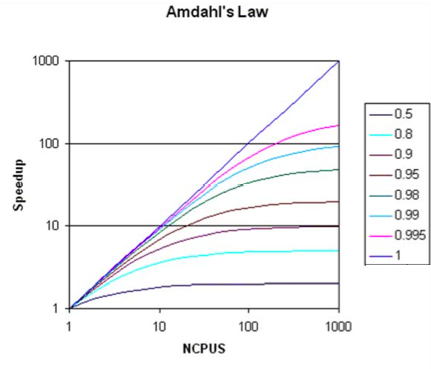
\includegraphics[height=250pt]{pics/amdahl}
  \captionof{figure}{Efficiency of Parallelization. On the right the fraction of parallelized time to total time.}
  \label{fig:amdahl}
\end{minipage}
\end{minipage}
\vspace{0.1cm}











